\section{Color Transparency at Intermediate Energies}
\label{sec:ct_intermediate_energies}

\subsection{Quasielastic proton scattering}
The first attempt to measure the onset of color transparency at energies where
significant expansion is expected took place at BNL.
These experiments measured nuclear transparency $T_{pp}$,
the ratio of the quasielastic cross section for a given target to the free $pp$
elastic cross section, for large-angle
($\SI{80}{\deg} < \theta_{cm} < \SI{90}{\deg}$) elastic $pp$ and quasielastic
$A(p,2p)$ scattering.
To account for Fermi motion and the fact that the square of the invariant
energy $s$ is different in quasielastic scattering and elastic scattering
from a free proton, transparency was measured as a function of the effective
incident momentum $p_{eff}$, defined by equation~\ref{eqn:ap2p_peff}.
\begin{equation} \label{eqn:ap2p_peff}
    s = 2 m_p \sqrt{m_p^2 + p_{eff}^2} + 2m_p^2
\end{equation}

The first experiment's measurements were taken using protons with incident
momenta of 6, 10, and \SI{12}{\giga\electronvolt} scatttering from carbon,
lithium, aluminum, copper, and lead targets~\cite{Carroll_1988}.
Nuclear transparency was observed to increase between $p_{eff}$ of 5.9 and
\SI{9.5}{\giga\electronvolt} and decrease above \SI{9.5}{\giga\electronvolt}.
A follow-up experiment~\cite{Mardor_1998, Leksanov_2001} extended these
carbon transparency measurements to \SI{14.5}{\giga\electronvolt}.
The results confirmed the behavior observed in the first experiment.
% The follow-up experiment also measured the angular dependence of $T_{pp}$.
The final transparency results from both experiments~\cite{Aclander_2004} are
shown in Figure~\ref{fig:ap2p} as a function of $p_{eff}$.
There are two proposed explanations for the observed rise and subsequent fall
in transparency.

\begin{figure}[!h]
    \centering
    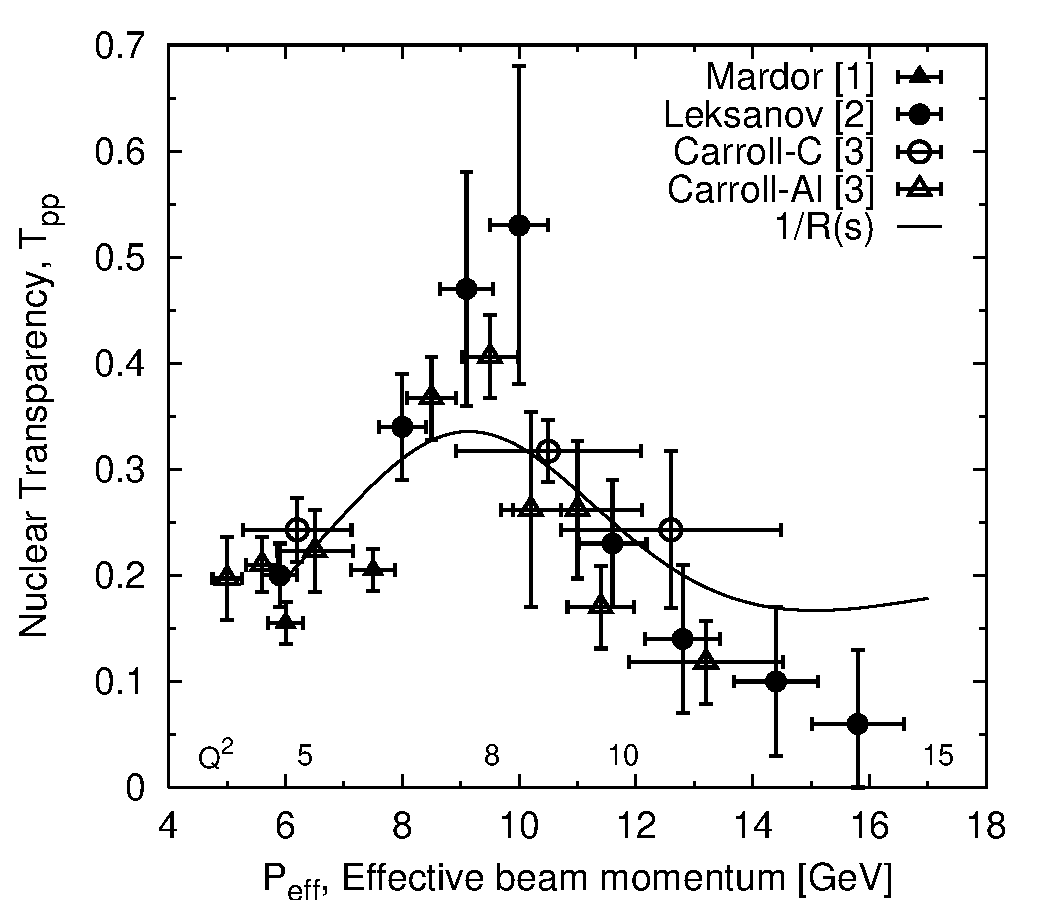
\includegraphics[width=0.6\textwidth]{chap2/ap2p.pdf}
    \caption{Transparency values $T_{pp}$ versus $p_{eff}$ for quasielastic
             proton scattering from carbon and aluminum (scaled by
             $(27/12)^{1/3}$) targets~\cite{Aclander_2004}.
             The solid curve is the inverse of $R(s)$ defined in
             equation~\ref{eqn:ap2p_rs}.
            }
    \label{fig:ap2p}
\end{figure}

\subsubsection{Interference between two terms}
One explanation focuses on interference between the amplitudes of two
perturbative QCD processes~\cite{Ralston_1988}, resulting in a transparency
that oscillates with $s$.
In this model, the effect of the energy-dependent phase shift on the scattering
amplitude can be respresented by
\begin{equation}
    M = M_{QC} + e^{i\phi(s) + i \delta_1}\left|M_L\right|
\end{equation}

Here $\delta_1$ is an energy-independent phase shift and $\phi(s)$ has a known
energy dependence analogous to renormalization-group
evolution~\cite{Pire_1982, Ralston_1982, Sen_1983}
\begin{equation}
    \phi(s) \propto \ln \ln \left( \frac{s}{\Lambda_{QCD}^2} \right)
\end{equation}


The first term $M_{QC}$ is a hard amplitude dominant at high energies,
characterizing quarks separated by small transverse
distances~\cite{Brodsky_1973, Brodsky_1975, Matveev_1973, Lepage_1980};
so-called ``quark counting rules'' predict that the asymptotic energy
dependence of $pp$ scattering at a fixed angle $\theta_{cm}$ should look like
$\frac{d\sigma}{dt}\sim s^{-10}$.
The second term $M_L$ is the Landshoff mechanism---three-gluon exchange in the
t-channel~\cite{Landshoff_1974, Landshoff_1980}.
It is suppressed at high energies, but may be significant at intermediate
energies~\cite{Mueller_1981}.


Taking the ratio of the differential cross section $d\sigma/dt$ to the
quark-counting prediction $d\sigma_0/dt$
yields the following ratio, with parameters $\rho_1$ and $K$ to be determined
by a fit to data:
\begin{align} \label{eqn:ap2p_rs}
    R(s) &= \frac{d\sigma}{dt_{pp}} \bigg/ \frac{d\sigma_0}{dt_{pp}}
          = s^{10} \frac{d\sigma}{dt_{pp}} \\
         &\propto 1 + \rho_1 s^{1-K} \cos\left[\phi(s)+\delta_1\right] + \rho_1^2 s^{2-2k}/4
\end{align}

\begin{figure}[!h]
    \centering
    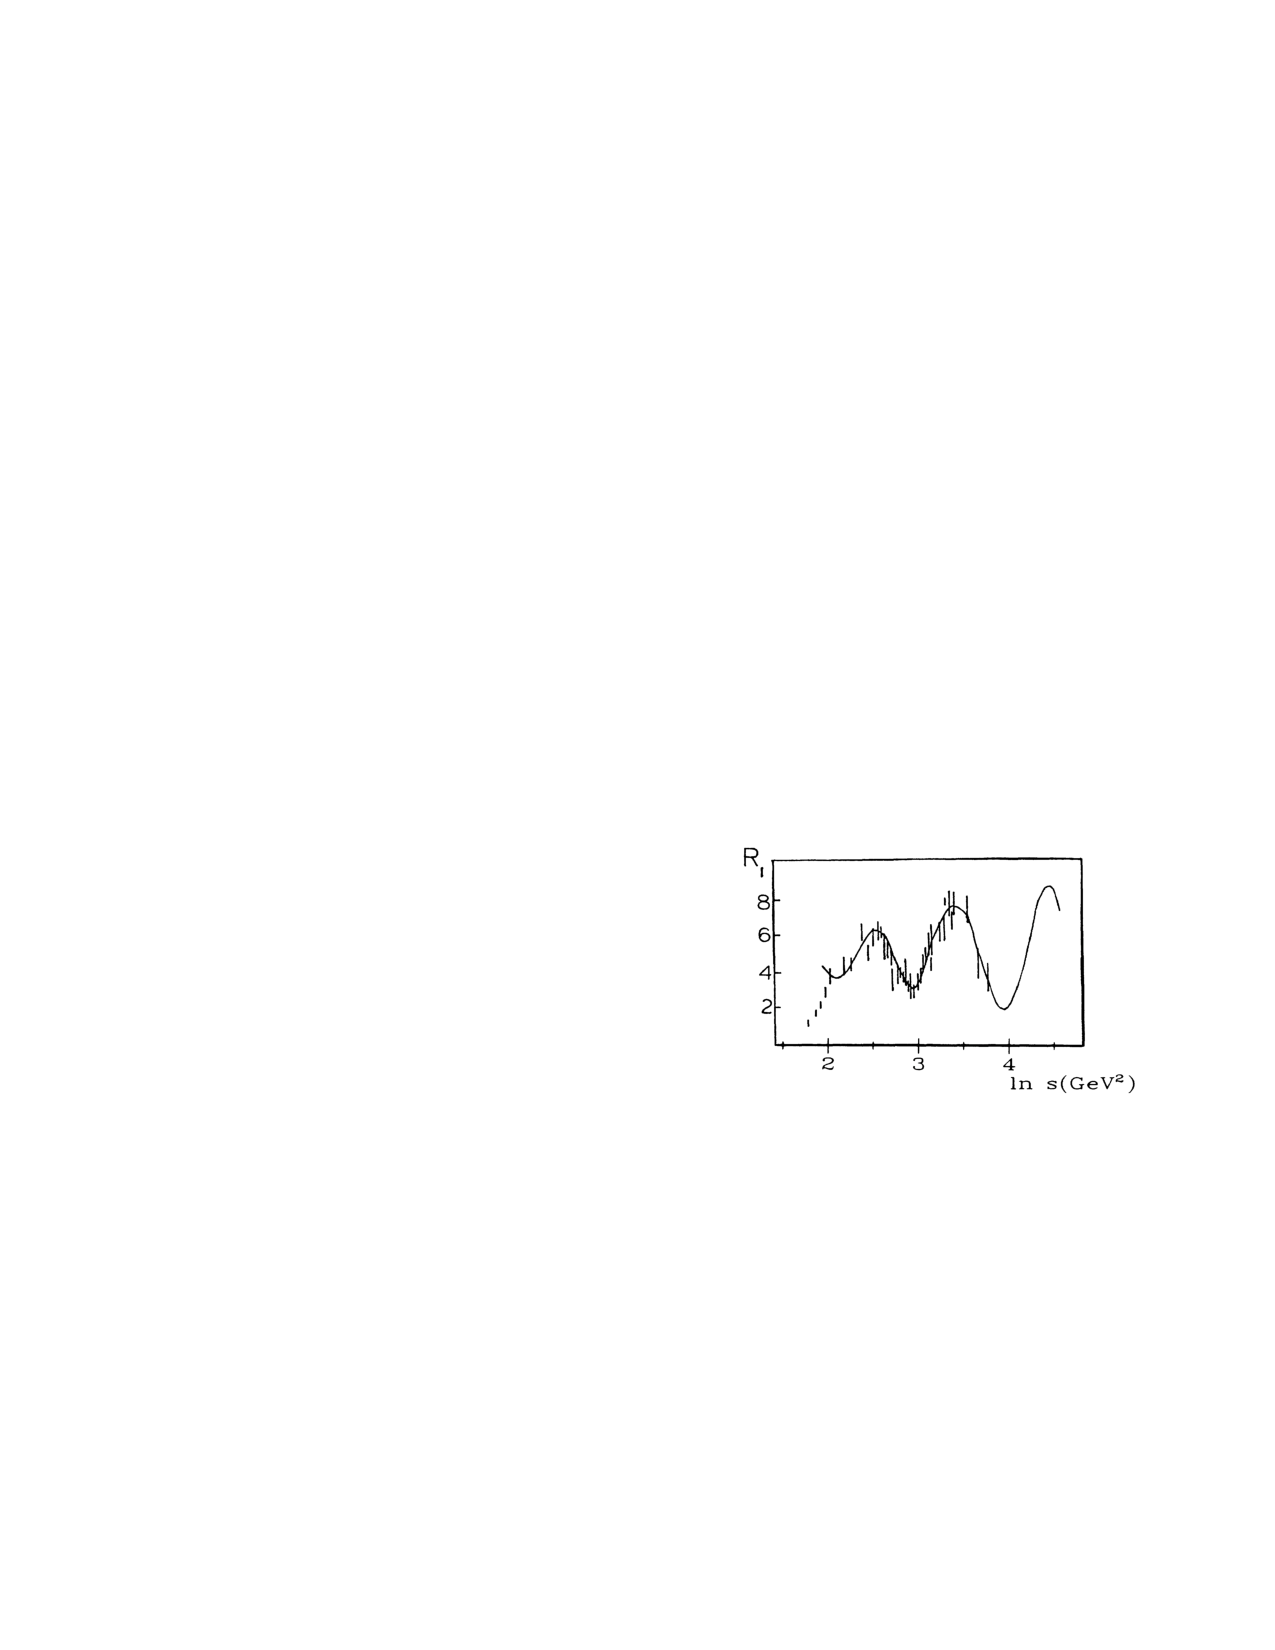
\includegraphics[width=0.6\textwidth]{chap2/pire_1982_R}
    \caption{A fit of $R(s)$, defined in equation~\ref{eqn:ap2p_rs}, to data taken from~\cite{Sivers_1976}
             for $pp$ elastic scattering at fixed angle
             $\theta_{cm}=\SI{90}{\deg}$.
             Figure reproduced from~\cite{Pire_1982}.
            }
    \label{fig:pire_1982_R}
\end{figure}

Similarly, this model predicts the energy dependence of the transparency $T$:
\begin{align}
    T(s) &= \frac{1}{A}\frac{d\sigma\left(pA \rightarrow pp(A-1)\right)/dt}
                            {d\sigma\left(pp \rightarrow pp\right)/dt} \\
         &\propto \frac{1 + \rho_A s^{1-K} \cos\left[\phi(s)+\delta_A\right] + \rho_A^2 s^{2-2k}/4}
                       {1 + \rho_1 s^{1-K} \cos\left[\phi(s)+\delta_1\right] + \rho_1^2 s^{2-2k}/4}
\end{align}


For large A such that $\rho_As^{1-K}\ll1$, the numerator is independent of
energy and transparency is approximately $1/R(s)$.
Given the form of $R(s)$ in equation~$\ref{eqn:ap2p_rs}$, the transparency
should oscillate as a function of $s$, with another rise potentially
appearing around $s\approx\SI{20}{\giga\electronvolt}$.

\subsubsection{New physics?}
The second explanation is that the energy dependence corresponds to a resonance
or some threshold for new physics, such as a charm quark resonance or some
multi-quark state.

\subsection{Quasielastic electron scattering}
Cleaner than A(p,2p) because both the electron-proton elastic scattering cross section
and spectral functions $S(p_m,E_m)$ for a variety of nuclei
have been measured extensively over a wide range of kinematics.
Complications involving $s$ near a charm threshold and oscillatory $s$
dependence mentioned in previous section are not relevant for A(e,e'p); for
quasielastic scattering $s$ is always approximately $m_p^2$.
This is also a scale where $\sigma_{tot}(pp)$ is relatively independent of $s$,
as shown in Fig~\ref{pdg_pp_cross_section}.

\begin{figure}[!h]
    \centering
    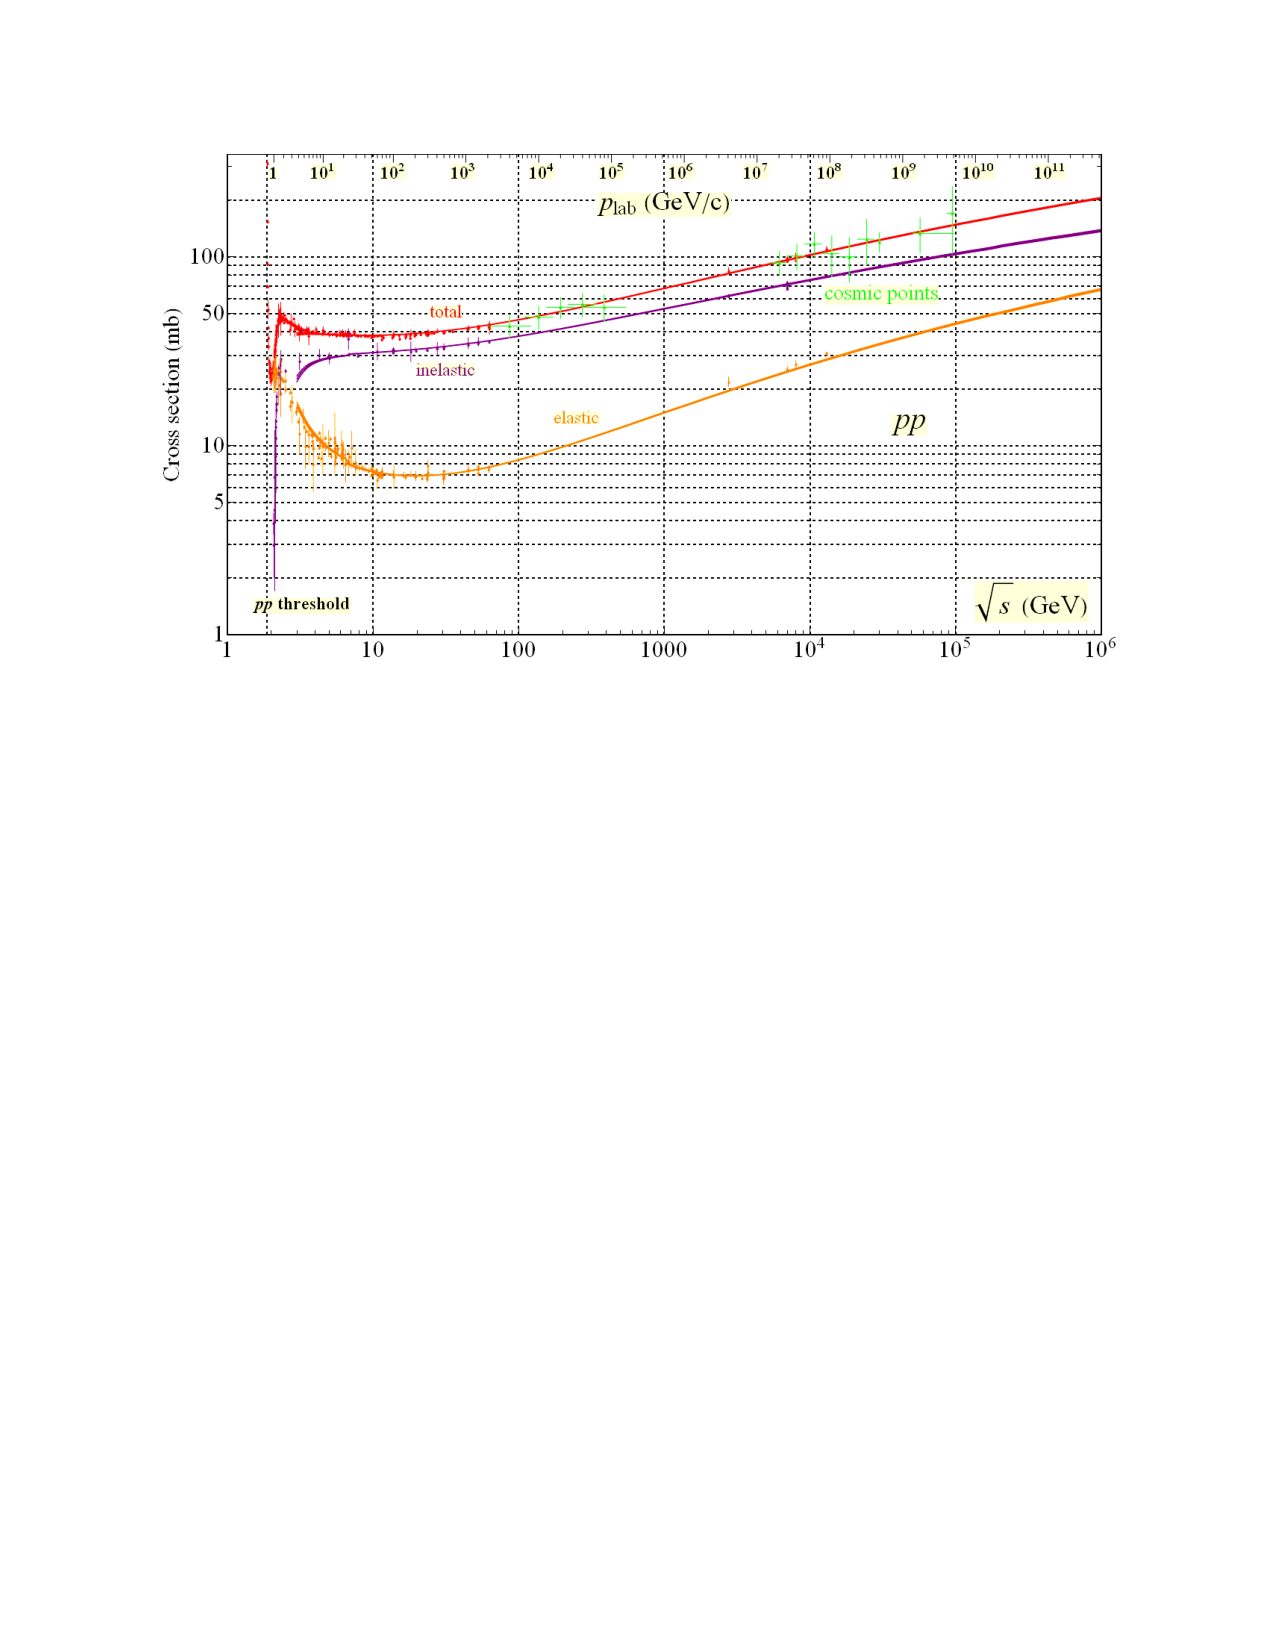
\includegraphics[width=0.6\textwidth]{chap2/pdg_pp_cross_section.pdf}
    \caption{
             Total, elastic, and inelastic $pp$ cross sections versus
             $p_{lab}$ and $sqrt{s}$.
             Note that the total cross section is relatively constant over the
             range of momenta studied in E12-06-107, about
             \SIrange{4}{10}{\giga\electronvolt}.
             Figure reproduced from Ref~\cite{pdg_2020}.
            }
    \label{fig:pdg_pp_cross_section}
\end{figure}

% TODO: expand here
Use the PWIA approximation to measure transparency

\begin{equation}
    T(Q^2) = \frac{\int_V \, d^3p_m \, dE_m \, Y_{exp}(E_m, \vec{p}_m)}
                  {\int_V \, d^3p_m \, dE_m \, Y_{PWIA}(E_m, \vec{p}_m)}
\end{equation}

Previous transparency measurements, compiled in Fig~\ref{fig:aeep}, were taken
at SLAC, MIT Bates, and JLab for several nuclear targets.
These transparency measurments are independent of $Q^2$ over the range of 2 to
\SI{8}{\giga\electronvolt}.
This is consistent with the Glauber prediction, which is to say, an absence of
color transparency.
%TODO: Cite the models.

% TODO: Do we have a PDF version of this?
\begin{figure}[!h]
    \centering
    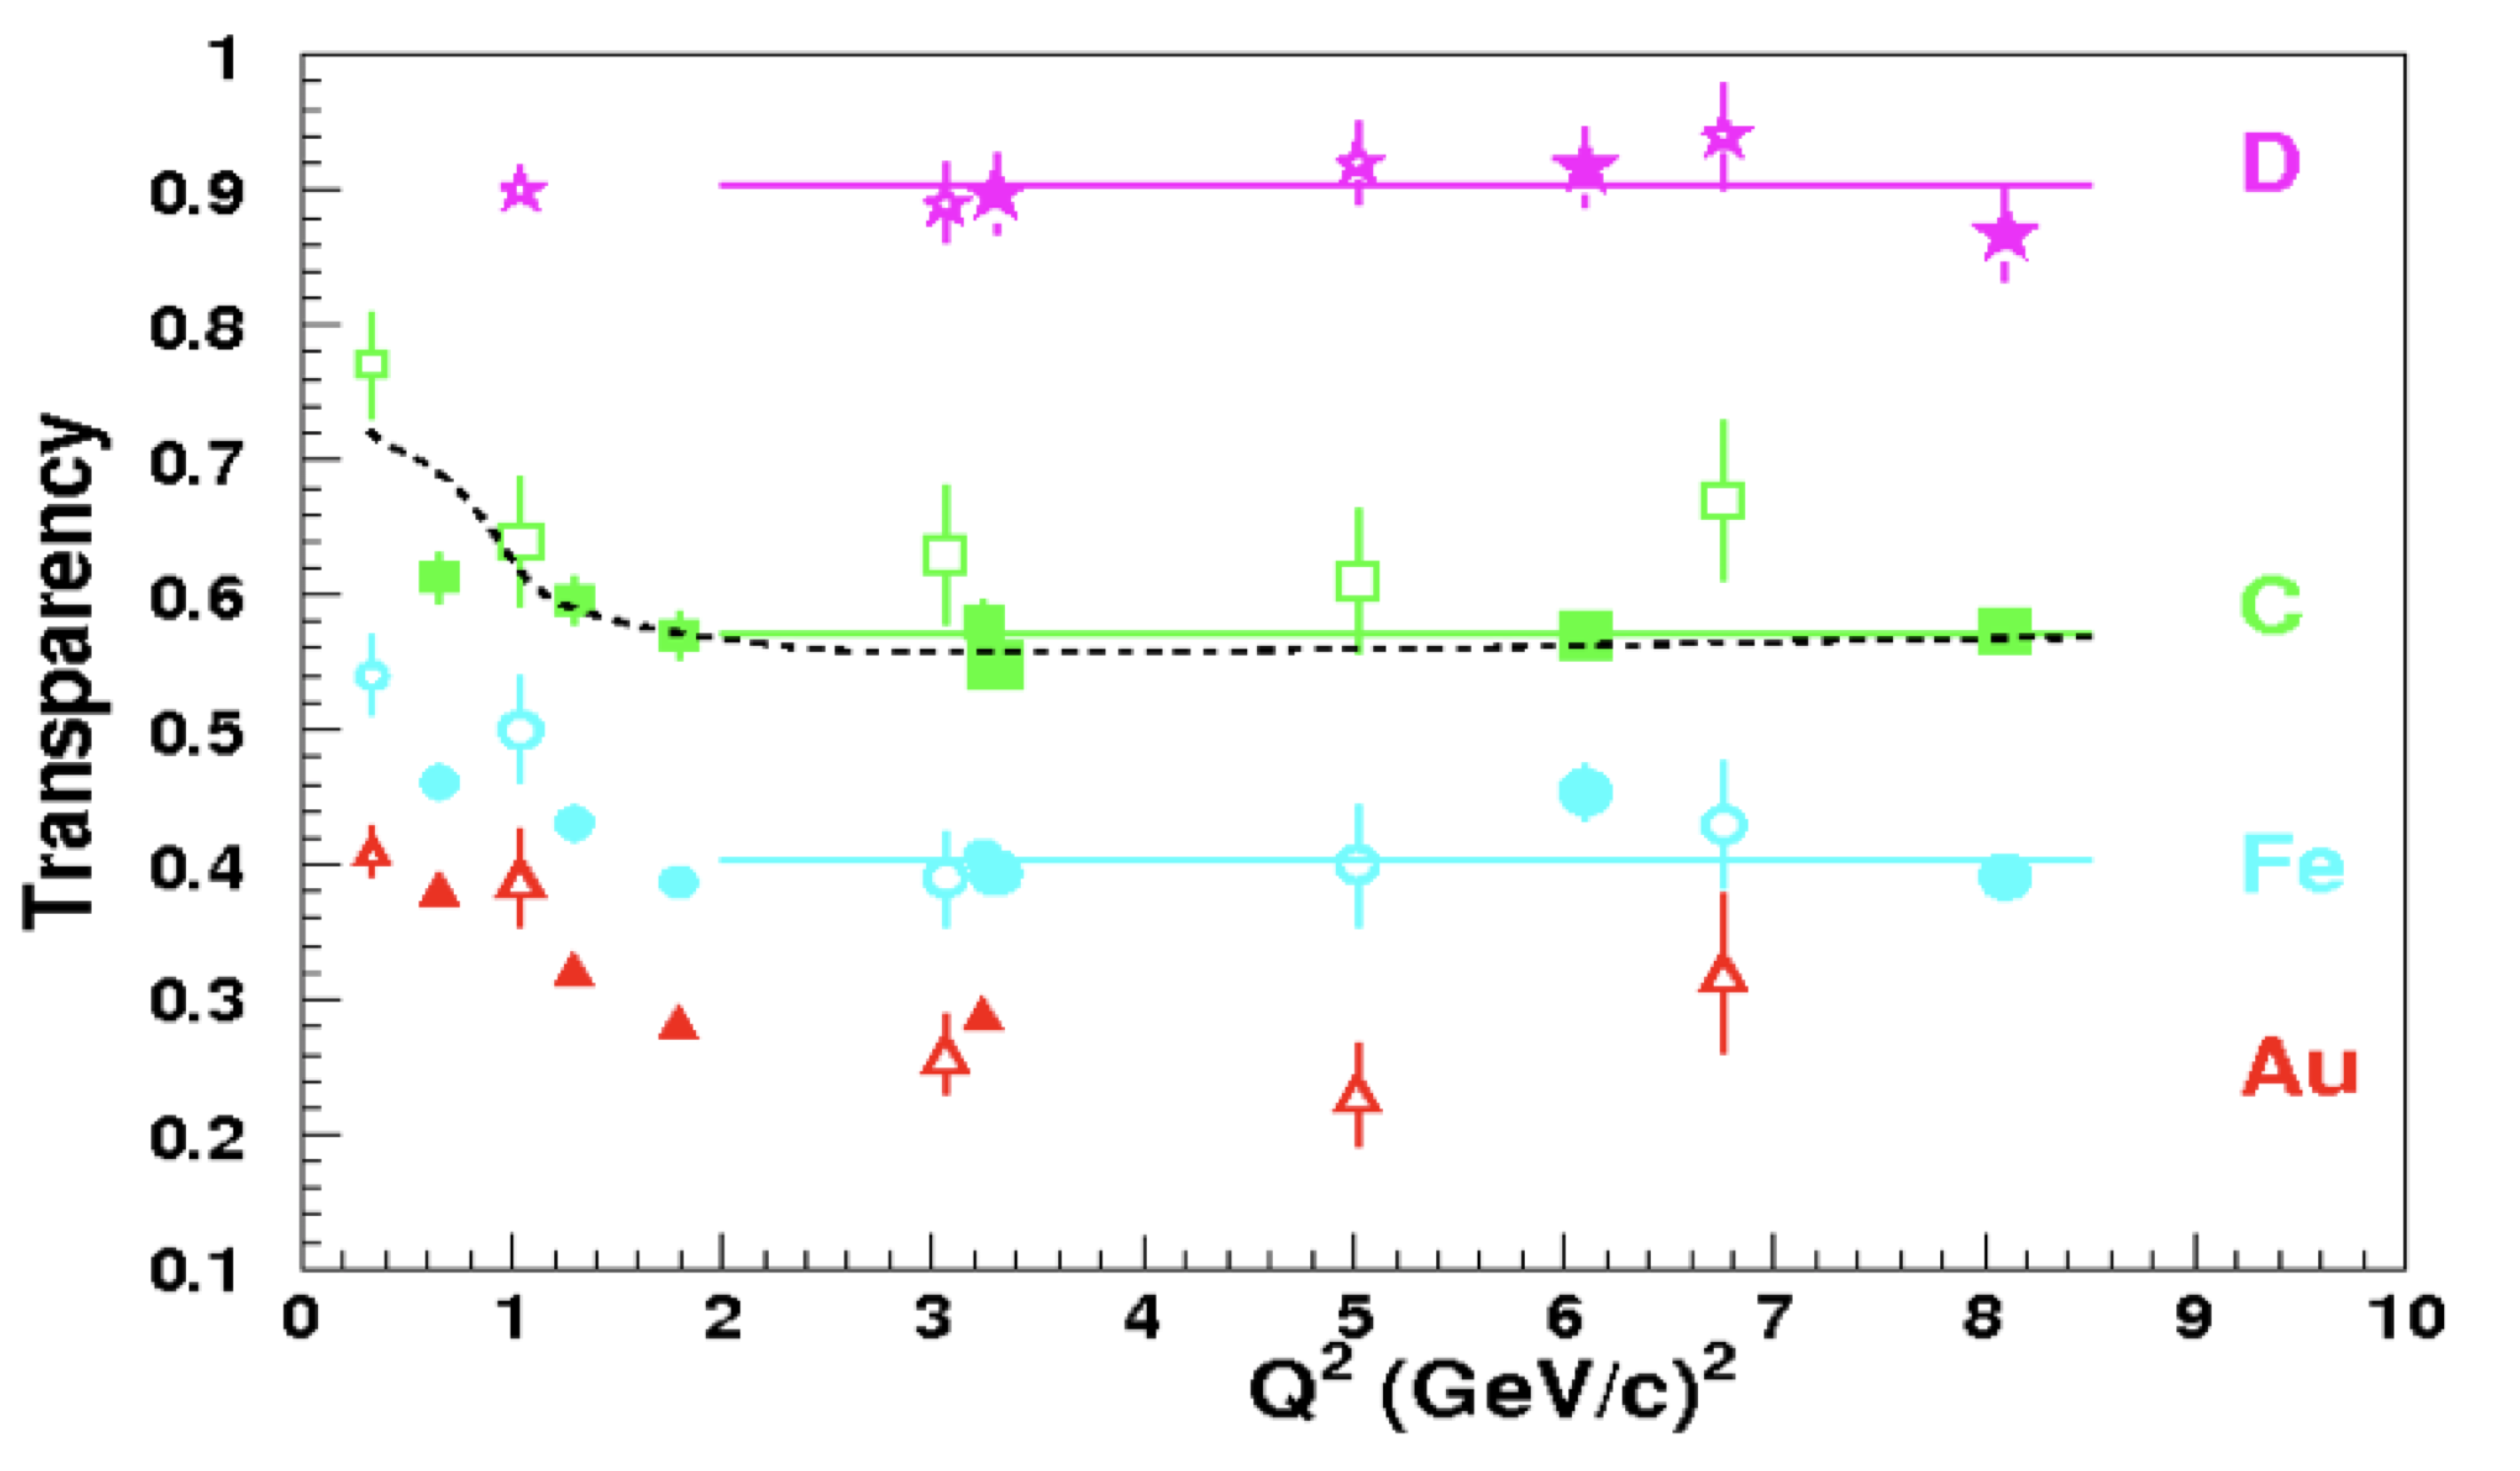
\includegraphics[width=0.6\textwidth]{chap2/aeep_transparency.png}
    \caption{Transparency measurements from several experiements studying
             quasielastic electron scattering from deuterium, carbon, iron,
             and gold.
             Data taken at JLab~\cite{Abbot_1998, Garrow_2002, Rohe_2005} are shown as solid points.
             Data taken at SLAC~\cite{Makins_1994, ONeill_1995} are shown as large open symbols.
             Data taken at Bates~\cite{Garino_1992} are shown as small open symbols.
             The dotted line is a Glauber calculation from~\cite{Pandharipande_1992} for carbon data..
             Solid lines are constant-value fits to data above \SI{2}{\giga\electronvolt}.
            }
    \label{fig:aeep}
\end{figure}


\subsection{Pion photoproduction}
The onset of color transparency in pion photoproduction was studied at JLab,
using Bremsstrahlung photons generated by the CEBAF beam incident on a copper
radiator~\cite{Dutta_2003}.
Transparency was mesured by taking the ratio of 4He to 2H cross sections at two
angles.
These measurements are shown in Fig~\ref{fig:pion_photoproduction_transparency}
along with two models.
The first model is a Glauber calculation, using exact ground state wave
functions~\cite{Arriaga_1995}.
The second adds CT to this model using the quantum diffusion model's modified hN
cross section~\cite{Farrar_1988}.

\begin{figure}[!h]
    \centering
    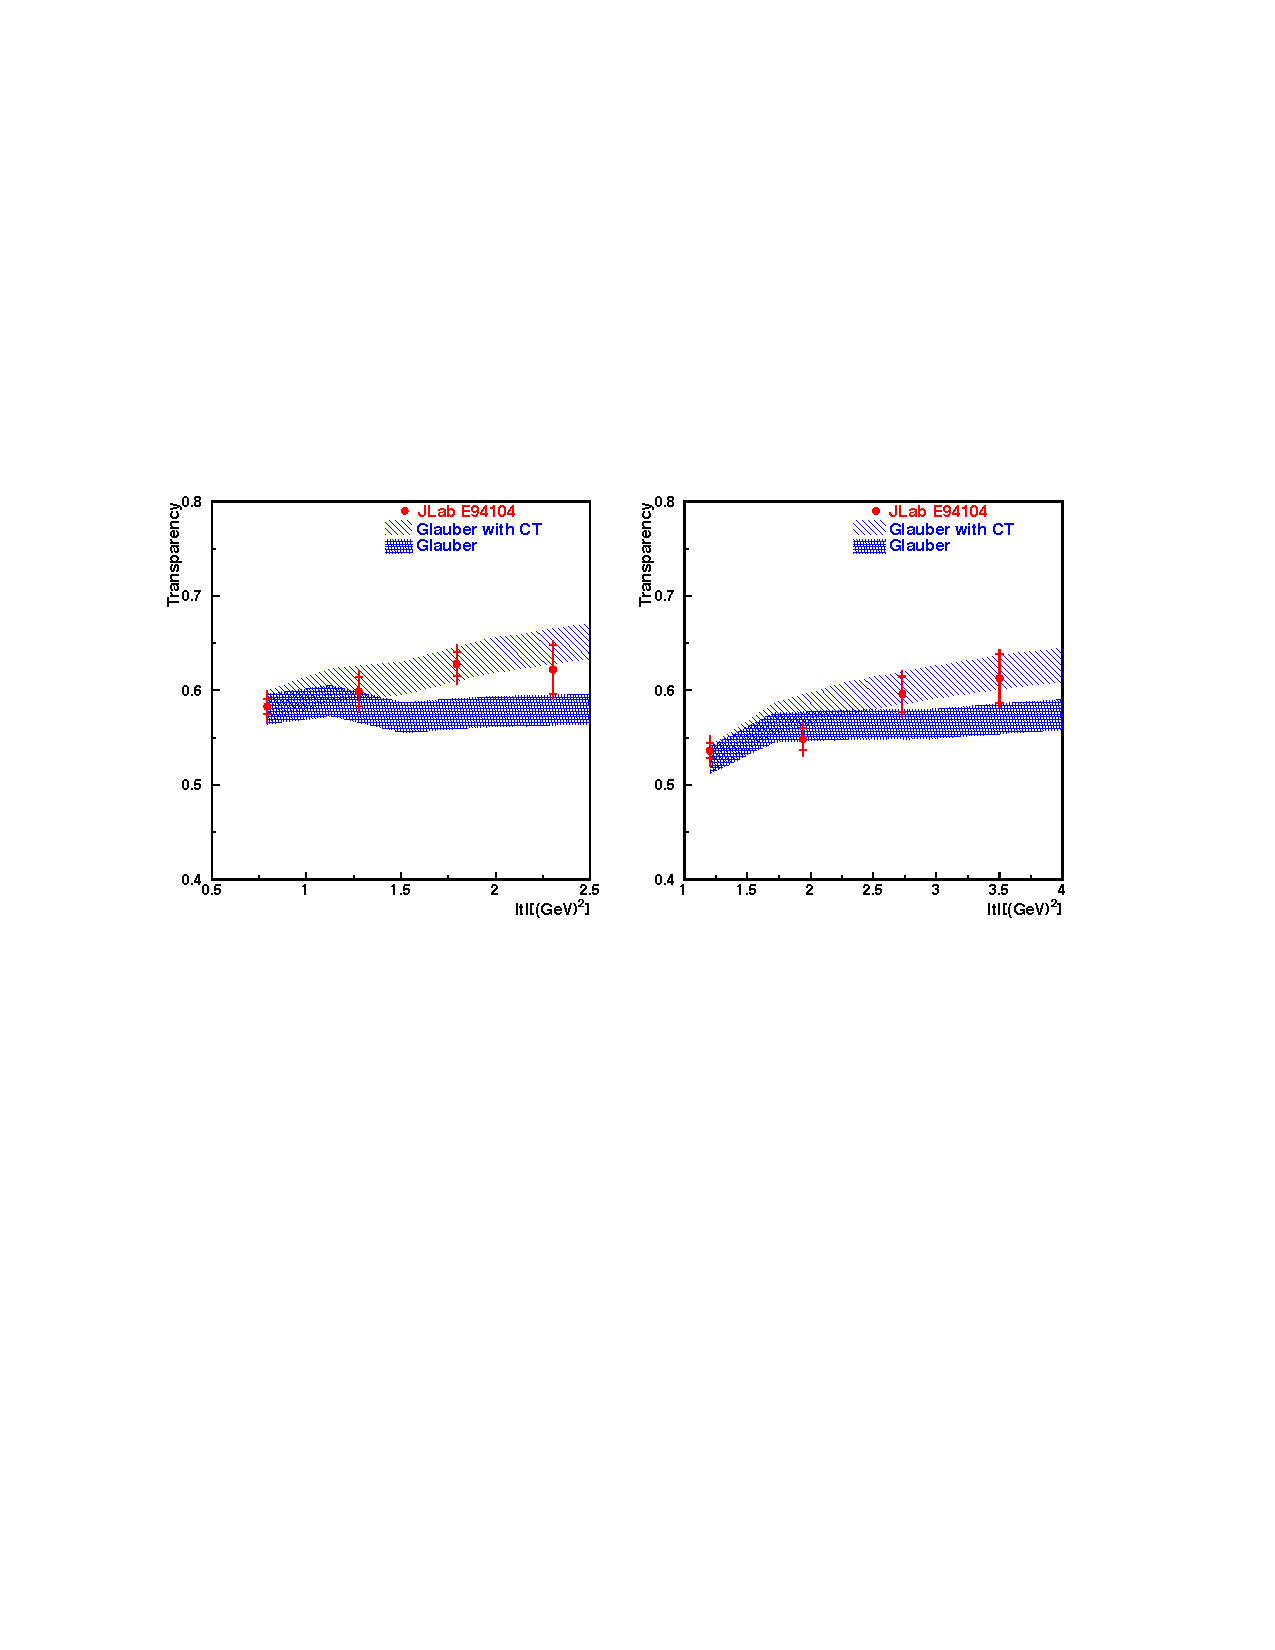
\includegraphics[width=0.6\textwidth]{chap2/pion_photoproduction_transparency.pdf}
    \caption{Nuclear transparency for $\ch{^{4}He}(\gamma,p\pi^+)$ at
            $\theta_{CM}=\ang{70}$ (left) and $\theta_{CM}=\ang{90}$ (right) as
            a function of 4-momentum transfer $\left|t\right|$.
            The inner bars are statistical uncertainties only.
            The outer bars are the statistical and point-to-point systematic
            uncertainties added in quadrature.
            The lower shaded band represents the prediction of a traditional
            Glauber calculation based on ground state wave functions for
            $\ch{^4He}$~\cite{Arriaga_1995}.
            The upper shaded band adds CT to this model using a modified
            hadron-nucleus cross section~\cite{Farrar_1988}.
            }
    \label{fig:pion_photoproduction_transparency}
\end{figure}

The slope of the measured transparencies' dependence on $Q^2$ is within 1sigma
(2sigma) of the Glauber calculation for the theta=70(=90) data.
The seem to deviate from the Glauber prediction, but a subsequent analysis using
a relativistic extension of the Glauber approximation showed that these data are
not conclusive evidence of the onset of CT \cite{Cosyn_2006}.


\subsection{Pion electroproduction}
The piCT experiment at JLab measured the $A$ and $Q^2$ dependence of the pion
cross section for several targets (\ch{^1H}, \ch{^2H}, \ch{^{12}C},
\ch{^{27}Al}, \ch{^{63}Cu}, and \ch{^{197}Au})~\cite{Clasie_2007, Qian_2010}.
Ref~\cite{Clasie_2007} defines nuclear transparency $T$ as the ratio of the pion
electroproduction cross section from a given nuclear target to the cross
section for a free proton, while Ref~\cite{Qian_2010} defines nuclear
transparency $T_D$ using the deuteron cross section in the denominator.
The purpose of this definition is to reduce uncertainty stemming from
the unknown pion electroproduction off a neutron and uncertainty in Fermi
smearing.
The deuterium nuclear transparency measurements are relatively independent of
$Q^2$, so both definitions show similar $Q^2$ dependencies in
Ref~\cite{Qian_2010}.
The transparency results are shown in
Fig~\ref{fig:pion_electroproduction_transparency_Q2_dependence} along with three
model predictions described below.

\begin{figure}[!h]
    \centering
    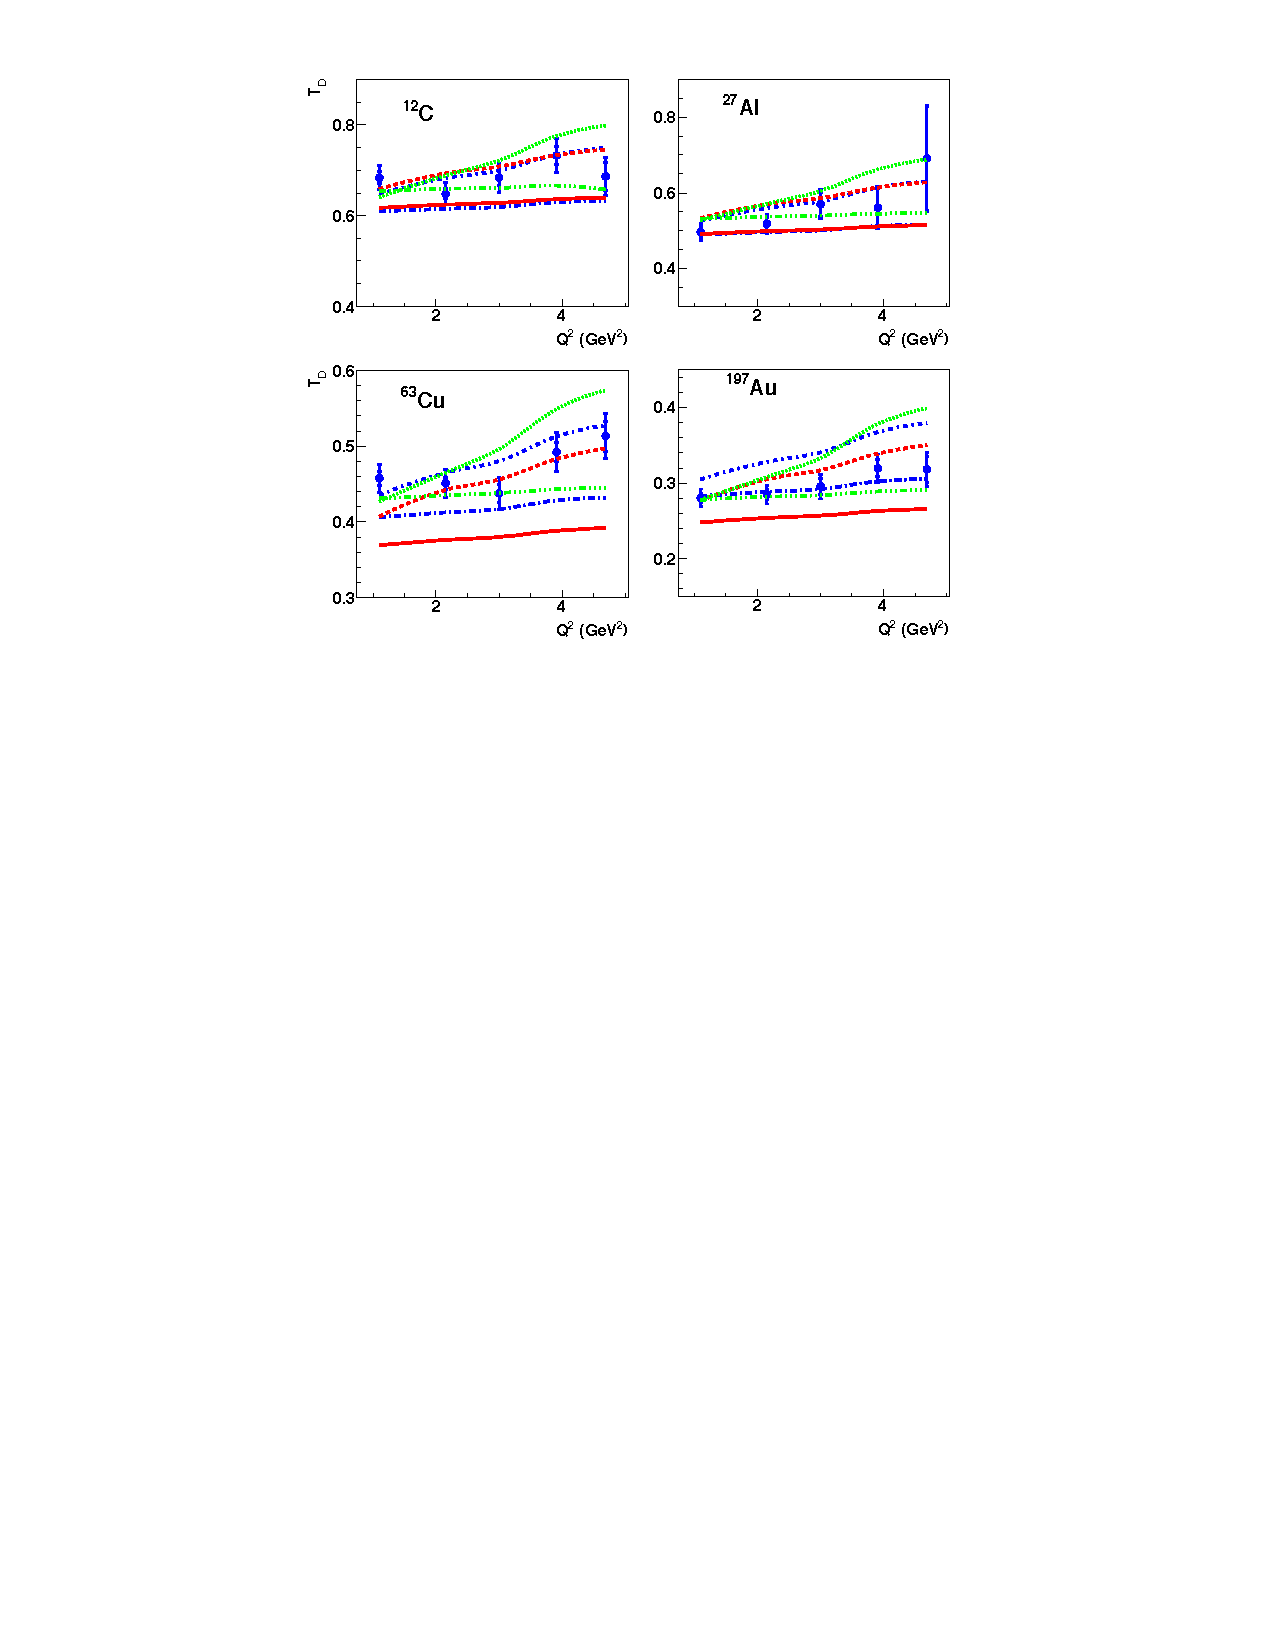
\includegraphics[width=0.6\textwidth]{chap2/pion_electroproduction_transparency_Q2_dependence.pdf}
    \caption{
            }
    \label{fig:pion_electroproduction_transparency_Q2_dependence}
\end{figure}

Larson et al.~\cite{Larson_2006} use a semiclassical formula based on the
eikonal approximation and a parameterization of final state interactions in
terms of an effective cross section based on a quantum diffusion
model~\cite{Farrar_1988}, in which the strength of the interaction is
proportional to the pion's propagation distance through the nucleus.
The transparency is given by a single integral over the path of the outgoing
pion, where the nuclear density $\rho(r)$ is of Woods-Saxon form,
\begin{equation}
    T = \frac{1}{A}\int d^3 \, r \rho(r)
           \exp{
                 -\int_z^\infty dz' \, \sigma_{eff} (z'-z,p_\pi) \rho(r')
               }
\end{equation}


Cosyn et al.~\cite{Cosyn_2008} calculate nuclear transparency as a ratio of
differential cross sections (integrated over the kinematic range of the
experiment) in a relativistic multiple scattering Glauber approximation (RMSGA)
to that in a relativistic plane wave impulse approximation (RPWIA).
All particles are taken to be plane waves in the RPWIA, while in the RMSGA
the wavefunctions of the outgoing pion and spectator nucleon are a convolution
of a plane wave with an eikonal phase operator that parameterizes the final
state interactions.
This model implements CT in this operator using the same quantum
diffusion model's effective cross section~\cite{Farrar_1988} used by Cosyn et
al.
This model also includes the effects of short range correlations, which create
local fluctuations in nuclear density.


Kaskulov et al.~\cite{Kaskulov_2009, Kaskulov_2012} calculate nuclear
transparency as a ratio of the differential cross sections from two variations
of the same model, one with and one without final state interactions.
This model is based on a microscopic description of pion
electroproduction from hydrogen~\cite{Kaskulov_2008}.
The nuclear reaction is broken up into hard partonic DIS and soft hadronic components.
It is assumed that the beam electron interacts with a
nucleon in the nucleus the way it would with a free nucleon (also taking into
account Fermi motion, Pauli blocking, and nuclear shadowing).
model of hadronization.
The time development of the PLC is determined by the quantum diffusion
model~\cite{Farrar_1988}, with formation and production times determined by
Monte Carlo simulation of the Lund string hadronization
model~\cite{Anderson_1983} as described in Ref~\cite{Gallmeister_2005}.
The produced hadrons are then propagated through the nuclear medium using the
Boltzmann-Uehling-Uhlenbeck (BUU) equation.
This propagation models elastic and inelastic rescattering of outgoing hadrons.


The results of this experiment are in agreement with the CT predictions of
Larson et al., while Cosyn et al. and Kaskulov et al. overestimate the $P_\pi$
and $Q^2$ dependence of the data.
Nevertheless, the observed increase in nuclear transparency is consistent with
CT.


In addition to studying the $Q^2$ dependence of nuclear transparency, this
experiment fit the data to the form $T=A^{\alpha(Q^2)-1}$ where $A$ is the
numebr of nucleons in the nucleus and $\alpha(Q^2)$ is a free parameter.
The results of this fit along with the predictions of Larson et al. and Cosyn et
al. are shown in Fig~\ref{fig:pion_electroproduction_transparency_A_dependence}.
These results show a clear difference from the prediction of the Glauber model
without CT.

\begin{figure}[!h]
    \centering
    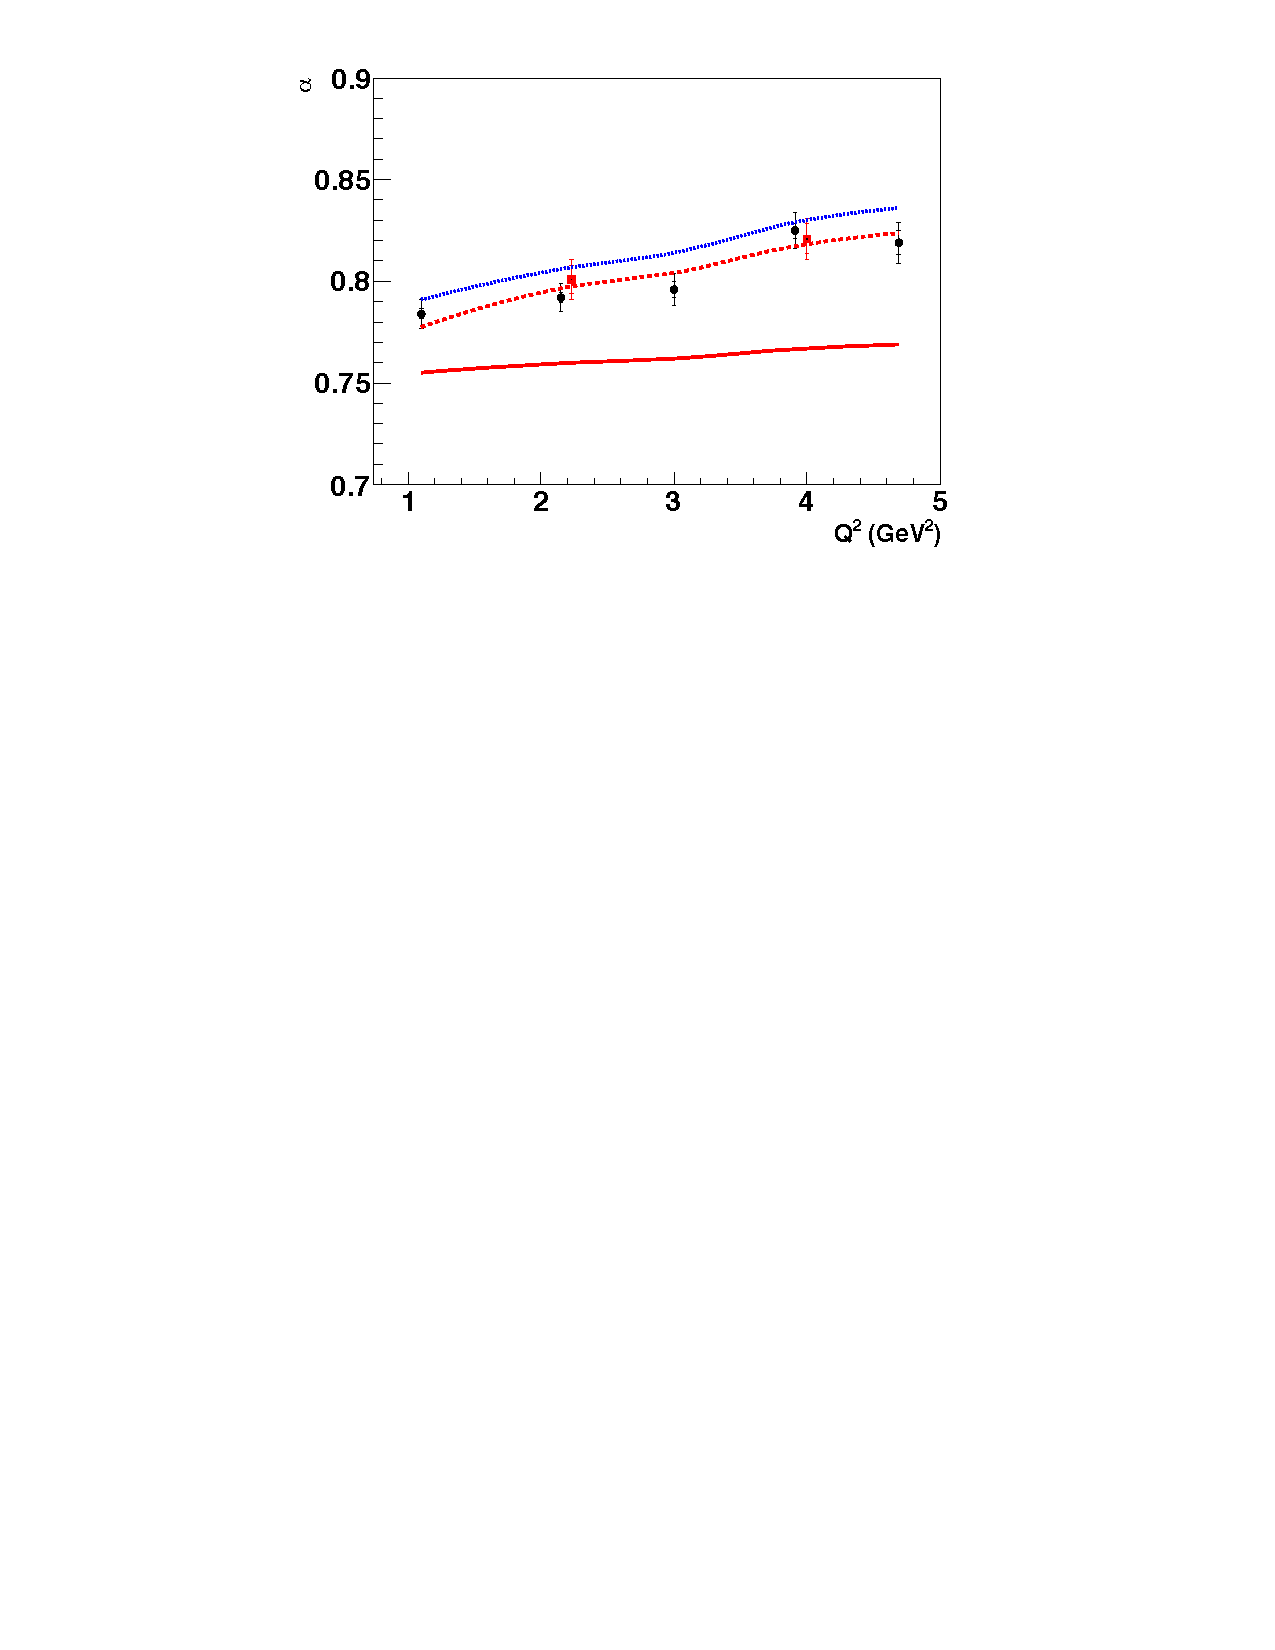
\includegraphics[width=0.6\textwidth]{chap2/pion_electroproduction_transparency_A_dependence.pdf}
    \caption{
            The parameter $\alpha(Q^2)$ extracted from a fit of nuclear
            transparency to form $T=A^{\alpha(Q^2)-1}$.
            The inner bars are statistical uncertainties only.
            The outer bars are the statistical, systematic, and model
            uncertainties added in quadrature.
            The solid, dashed and dotted lines are the predictions of
            the Glauber model of Ref~\cite{Larson_2006},
            the Glauber+CT model of Ref~\cite{Larson_2006},
            and the Glauber+CT+SRC model of Ref~\cite{Cosyn_2006},
            respectively.
            }
    \label{fig:pion_electroproduction_transparency_A_dependence}
\end{figure}

\subsection{$\rho^0$ meson leptoproduction}
Because of the hadronic structure of high energy photons,
a virtual can fluctuate to a smalll $q\bar{q}$ state with mass $M_qq$ and
propagate through a nucleus.
The formation length $l_{fr}=2\nu/(Q^2+M^2_qq)$ refers to the distance over
which this $q\bar{q}$ state is frozen.
The coherence length $l_c=2\nu/(m^2_{v'}-m^2_{v})$ refers to the distance over
which the small $q\bar{q}$ state grows to a normal size $\rho^0$ meson,
where $m_v$ is the mass of the $\rho^0$ in its ground state
and $m_{v'}\approx\SI{1.5}{\giga\electronvolt}$ is the mass of the lowest $\rho$
excited state.


The results of early exclusive diffractive $\rho_0$ leptoproduction
experiments in the 1990s were suggestive of the onset of CT, but had limited
statistical power.
Another factor complicating the study of CT in this exclusive process is the
need to separate the effects of $l_{fr}$ and $l_c$.
If one is not careful, an increase in nuclear transparency with decreasing
$l_{fr}$ can be mistaken for an increase with $Q^2$, the signature of CT.


The first measurements of nuclear transparency for incoherent diffractive
$\rho^0$ leptoproduction were performed
at Fermilab by the E665 collaboration \cite{Adams_1995} and
at CERN by the NMC collaboration \cite{Arneodo_1994}
using muon beams of \SI{450}{\giga\electronvolt} and
\SI{200}{\giga\electronvolt} respectively.
At these energies, the $l_{fr}$ is comparable to the nuclear radius and
the $l_c$ is much larger than the nuclear radius; the $q\bar{q}$
state is frozen.
E665 took data with XYZ targets, while NMC took data with XYZ targets.
The results for carbon and calcium, shown together in Fig(ref), are consistent
with each other and show a slight increase in transparency.
This is only suggestive of an onset of CT due to limited statistics and
substantial background.


E665 also studied the $A$-dependence of the cross section, fitting their data
for all targets to a power law, $\sigma_A=\sigma_0A^\alpha(Q^2)$ where both
$\sigma_0$ and $\alpha$ are free parameters.
The extracted value of $\alpha$ at low $Q^2$ is consitent with soft nuclear
interactions.
The increase of $\alpha$ at higher $Q^2$ is again only suggestive of CT due to
the large uncertainty.


The HERMES collaboration at DESY~\cite{Ackerstaff_1999} measured nuclear
transparency as a function of $Q^2$ and $l_{fr}$ for coherent and incoherent
$\rho^0$ leptoproduction from \ch{^{14}N} using a \SI{27.5}{\giga\electronvolt}
positron beam.
Their measurements for exclusive incoherent electroproduction, shown in
Fig(ref), show an increase in transparency at lower $l_{fr}$ consistent with an
introduction of initial state interactions between the nuclear medium and the
$q\bar{q}$ pair (i.e. when the pair remains small for a distance smaller than
mean free path of a $\rho^0$ meson.)


Because $l_{fr}$ is comparable the nuclear radius in this experiment, these
measurements depend on $l_c$.
As such, the collaboration studied the nuclear tranparency's $Q^2$-dependence
while keeping $l_{fr}$ fixed.
Transparencies were extracted for fixed $(l_{fr},Q^2$ bins, as shown in
Fig(ref).
Due to low statistics, the transparencies were fit to a form
$P_0 + P_1 \cdot Q^2$, where $P_0$ is a free parameter for each $l_fr$ bin and
the slope $P_1$ is a common free parameter among the bins.


The extracted slopes for incoherent and coherent production were $0.70\pm0.21$
and \SI{0.089\pm0.046}{\per\giga\electronvolt\squared} respectively.
These slopes agree with the predictions of a model using the light cone Green
function formalism, incorporating the effects of coherence length and
CT~\cite{Kopeliovich_2002}.
As with the E665 and NMC results, the HERMES results are only suggestive of the
onset of CT due to their limited statistics.


The CLAS collaboration measured nuclear transparency for exclusive
incoherent $\rho^0$ production off carbon and iron relative to deuterium using
a \SI{5}{\giga\electronvolt} electron beam at JLab~\cite{ElFassi_2012}.
% The $t$ distributions were fit to a form $Ae^{-bt}$.
These transparencies are shown as a function of $l_{fr}$ in Fig(ref).
As seen in Fig(ref), these transparencies are independent of $l_{fr}$ because
$l_{fr}$ (\SIrange{\sim0.5}{0.9}{\femto\meter}) is smaller than the nuclear
radii of carbon and iron, \SI{2.9}{\femto\meter} and \SI{4.6}{\femto\meter}
respectively.
As a result, any increase in transparency as a function of $Q^2$ cannot be a
result of varying $l_{fr}$, but rather a signal of CT.


The $Q^2$ dependence of these transparency measurements is shown in Fig(ref)
along with the predictions of two models.
The Frankfurt-Miller-Strikman (FMS) model~\cite{Frankfurt_2008} uses a standard
Glauber calculation, using the quantum diffusion model's modified
hadron-nucleus cross section~\cite{Farrar_1988} to implement CT. This model
also includes the effects of the decay of the $\rho^0$ meson.
The Gallmestier-Kaskulov-Mosel (GKM) model~\cite{Gallmeister_2011} is similar
to Kaskulov et al.'s model~\cite{Kaskulov_2008} of pion electroproduction,
which uses the BUU formalism to transport (pre)hadrons through the nucleus.
Both models predict the behavior of the CLAS carbon data quite well, but the
GKM modek underestimates the iron transparency.


These data were also fit to a linear form $T=aQ^2+b$,
and the slope $a$ was compared to the predictions of the above two models as
well as a third, the Kopeliovich-Nemchick-Schmidt (KNS)
model~\cite{Kopeliovich_2007}.
The KNS model uses the same light cone Green function formalism used in the
context of the HERMES $\rho^0$ production data.
The results of these fits and the model predictions are shown in
Table~\ref{tab:CLAS_slopes}.

\begin{table}[h]
    \centering
    \label{tab:CLAS_slopes}
    \caption{
            Slope parameters from a fit to the $Q^2$ dependence of CLAS
            nuclear transparency data taken for carbon and
            iron~\cite{ElFassi_2012}. Also shown are predictions of the
            KNS~\cite{Kopeliovich_2007},
            GKM~\cite{Gallmeister_2011}, and
            FMS~\cite{Frankfurt_2008} models.
            }
    \begin{tabular}{ccccc}
        \hline
         Nucleus &  Measured slopes (\si{\per\giga\electronvolt\squared}) & \multicolumn{3}{c}{Model predictions} \\ \cline{3-5}
                 &                                                        &  KNS  &  GKM  &  FMS                  \\ \hline
         C       &  $0.044\pm0.015_{stat}\pm0.019_{sys}$                  & 0.06  & 0.06  & 0.025                 \\
         Fe      &  $0.053\pm0.008_{stat}\pm0.013_{sys}$                  & 0.047 & 0.047 & 0.032                 \\ \hline
    \end{tabular}
\end{table}
